\documentclass{article}
\usepackage{float}
\usepackage{graphicx}
\usepackage{geometry}
\addtolength{\topmargin}{-.875in}
\addtolength{\textheight}{1.75in}

\begin{document}
\def\mca#1{\multicolumn{1}{c}{#1}}
\def\mcb#1{\multicolumn{1}{c|}{#1}}
\renewcommand{\arraystretch}{2.25}

\begin{center}
{\large Grades 4/5}
\end{center}

1. In {\bf Times Out} puzzle, the goal is to place numbers in a square grid so that there are exactly two numbers in each row and two numbers in each column. Some of the rows and columns have clues. A number to the left of the grid gives the product of numbers in that row. Similarly, a number above the grid gives the product of the two numbers in that column. In 3x3 puzzles, each digit 1-6 should be used exactly once. In 4x4 puzzles, each digit 1-8 should be used exactly once.
\vspace{3mm}

Example: Solve the following Times Out puzzle.

\begin{tabular}{p{5mm}|p{5mm}|p{5mm}|p{5mm}|}
  \mca{}  & \mca{10} & \mca{18} & \mca{} \\\cline{2-4}
  \mcb2   &     &    &     \\\cline{2-4}
  \mcb{}  &     &    &     \\\cline{2-4}
  \mcb{24} &    &    &     \\\cline{2-4}
\end{tabular}
\vspace{3mm}

Solution: For all numbers in the table, there is only one way to write them as products of two numbers, each of them at most 6:

2 = 2 x 1, 10 = 2 x 5, 18 = 3 x 6, 24 = 4 x 6

Since both the column marked by 10, and the row marked by 2 must contain 2, it must be in their intersection. Similarly, 18-column and 24-row must contain 6, hence it is in their intersection.

\begin{tabular}{p{5mm}|p{5mm}|p{5mm}|p{5mm}|}
  \mca{}  & \mca{10} & \mca{18} & \mca{} \\\cline{2-4}
  \mcb2   & 2  &    &     \\\cline{2-4}
  \mcb{}  &    &    &     \\\cline{2-4}
  \mcb{24} &   & 6  &     \\\cline{2-4}
\end{tabular}
\vspace{3mm}

We must place $3$ in the 18-column, but not 2-row (since 3 does not divide 2), hence it must be in the middle. Since there are already 2 numbers in the 18-column, 1 (from 2x1 = 2) must be in the third column and 2-row.

\begin{tabular}{p{5mm}|p{5mm}|p{5mm}|p{5mm}|}
  \mca{}  & \mca{10} & \mca{18} & \mca{} \\\cline{2-4}
  \mcb2   & 2  &    & 1   \\\cline{2-4}
  \mcb{}  &    & 3  &     \\\cline{2-4}
  \mcb{24} &   & 6  &     \\\cline{2-4}
\end{tabular}
\vspace{3mm}

We must place $4$ in 24-row but not 10-column - hence it must be in the third column. It remains to place 5 - it must be in 10-column but not 24-row, hence it must be in the middle row.

\begin{tabular}{p{5mm}|p{5mm}|p{5mm}|p{5mm}|}
  \mca{}  & \mca{10} & \mca{18} & \mca{} \\\cline{2-4}
  \mcb2   & 2  &    & 1   \\\cline{2-4}
  \mcb{}  & 5  & 3  &     \\\cline{2-4}
  \mcb{24} &   & 6  & 4   \\\cline{2-4}
\end{tabular}
\vspace{3mm}

Solve the following Times Out puzzles.

\begin{tabular}{p{5mm}|p{5mm}|p{5mm}|p{5mm}|}
  \mca{}  & \mca{12} & \mca{} & \mca{6} \\\cline{2-4}
  \mcb{20}   &     &    &     \\\cline{2-4}
  \mcb{}  &     &    &     \\\cline{2-4}
  \mcb{12} &    &    &     \\\cline{2-4}
\end{tabular}
\begin{tabular}{p{5mm}|p{5mm}|p{5mm}|p{5mm}|}
  \mca{}  & \mca{5} & \mca{18} & \mca{} \\\cline{2-4}
  \mcb{6}   &     &    &     \\\cline{2-4}
  \mcb{}  &     &    &     \\\cline{2-4}
  \mcb{30} &    &    &     \\\cline{2-4}
\end{tabular}
\vspace{3mm}

\begin{tabular}{p{5mm}|p{5mm}|p{5mm}|p{5mm}|p{5mm}|}
  \mca{}  & \mca{7} & \mca{40} & \mca{} & \mca{6} \\\cline{2-5}
  \mcb{3} &     &    &    &  \\\cline{2-5}
  \mcb{}  &     &    &    & \\\cline{2-5}
  \mcb{12} &    &    &    & \\\cline{2-5}
  \mcb{35} &    &    &    & \\\cline{2-5}
\end{tabular}
\begin{tabular}{p{5mm}|p{5mm}|p{5mm}|p{5mm}|p{5mm}|}
  \mca{}  & \mca{8} & \mca{24} & \mca{15} & \mca{} \\\cline{2-5}
  \mcb{56} &     &    &    &  \\\cline{2-5}
  \mcb{}  &     &    &    & \\\cline{2-5}
  \mcb{12} &    &    &    & \\\cline{2-5}
  \mcb{6} &    &    &    & \\\cline{2-5}
\end{tabular}
\begin{tabular}{p{5mm}|p{5mm}|p{5mm}|p{5mm}|p{5mm}|}
  \mca{}  & \mca{35} & \mca{} & \mca{8} & \mca{24} \\\cline{2-5}
  \mcb{8} &     &    &    &  \\\cline{2-5}
  \mcb{}  &     &    &    & \\\cline{2-5}
  \mcb{12} &    &    &    & \\\cline{2-5}
  \mcb{28} &    &    &    & \\\cline{2-5}
\end{tabular}
\vspace{5mm}

2. Guess my number. A teacher plays the following game with 3 students - Alice, Bob, and Charlie. She writes numbers 1, 2, 3, 4 on four sticky notes, then places one sticky note at each student's forehead, and hides one in her pocket.
\vspace{3mm}

2A. The teacher asks Alice, "Is your number odd or even?". Alice looks at other students and says, "Even.". What numbers do Bob and Charlie have on their foreheads?
\vspace{3mm}

2B. The teacher takes of the sticky notes, rearranges them, and places them on the students' foreheads again. She then asks Bob, "Is your number greater than 2"? Bob says "Yes."

a) What numbers do Alice and Charlie have?

b) The teacher then asks Charlie, "What number is on your head?". Charlie says "One.". What number is on Alice's head?
\vspace{3mm}

2C. The teacher takes of the sticky notes, rearranges them again, and puts them back on the students' foreheads. He asks Charlie, "Is your number larger or smaller than Alice's?". Charlie says, "I can't tell."

a) What numbers can't be on Alice's forehead?

b) The teacher then asks Bob, "What number is on your head?" Bob answers "Four!" What number does Alice have?

c) What number is in the teacher's pocket?
\vspace{5mm}

3. Drew has a box of 50 toy cars. There are 18 cars that are red, and there are 7 cars that are missing at least one wheel. Three of the red cars are missing a wheel. How many cars in Drew's box are not red and are not missing any wheels?
\vspace{5mm}

4. In the diagrams below, the arrows of the same color stand for the same number. The following must hold: "value at arrow start" + "arrow value" = "value at arrow target". For example, $2 \rightarrow 5$ means that the arrow stands for "3". Fill in the missing numbers, and find out the arrow value for each color.

\begin{figure}[H]
  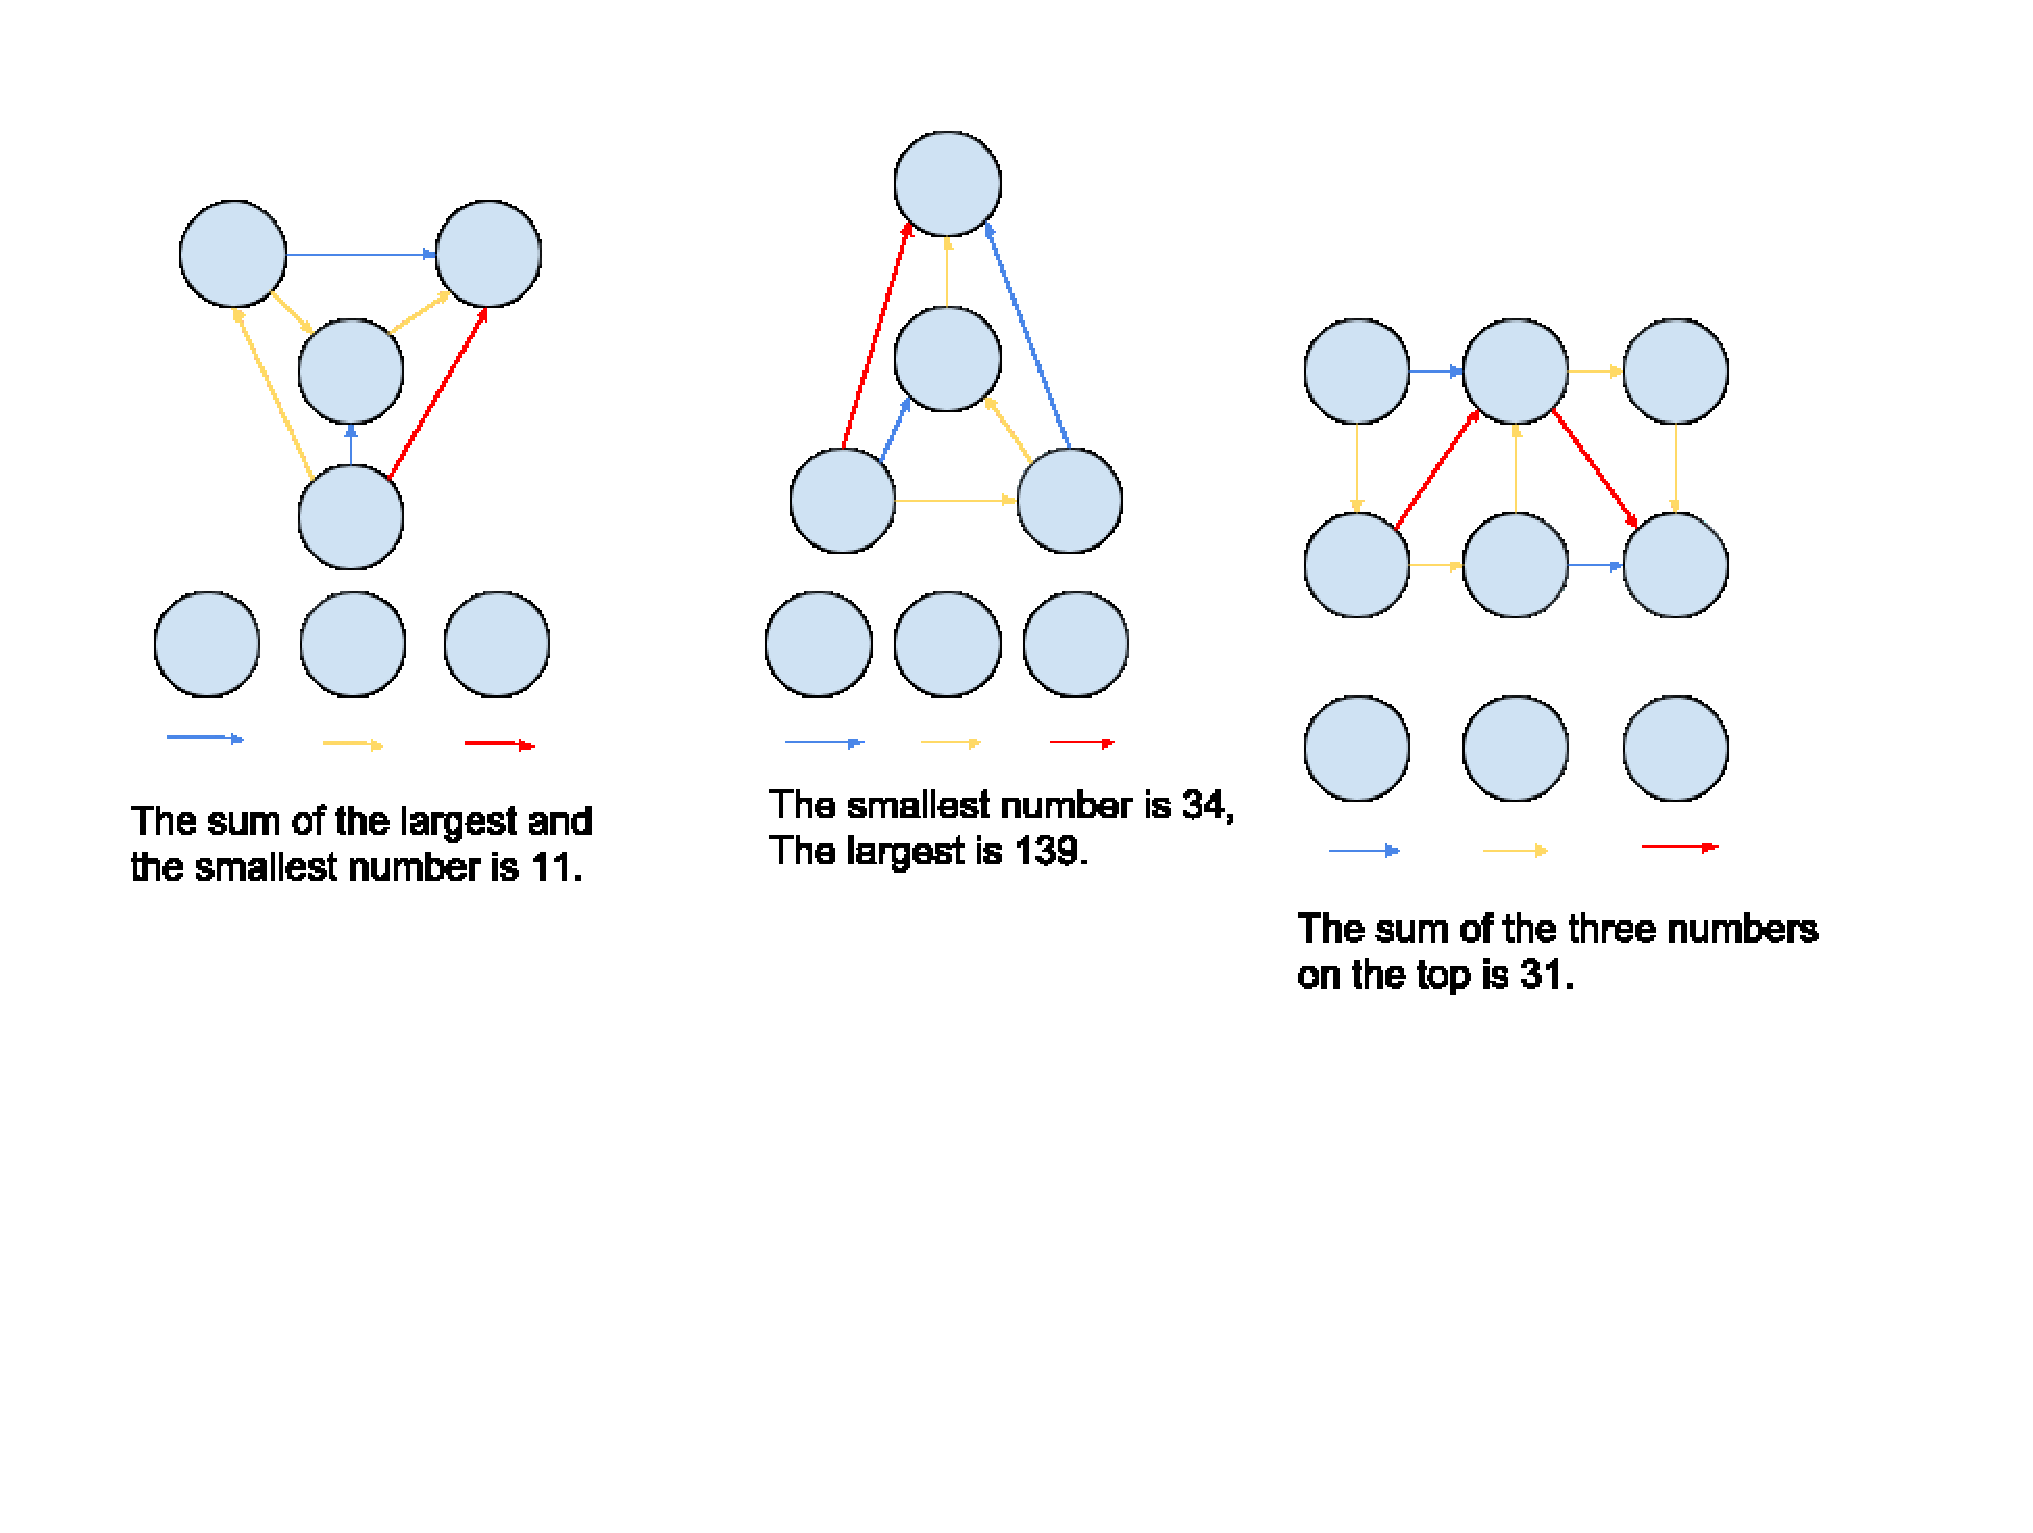
\includegraphics[width=0.8\textwidth]{pavuciny45.eps}
\end{figure}

5. In a {\bf Sum Square} puzzle, the digits 1 through 9 (positive or negative) are used in the 9 squares of the grid, one digit per square. The numbers above and to the left from the grid indicate the sums of numbers in columns and rows. Fill in the missing numbers.

\begin{tabular}{p{5mm}|p{5mm}|p{5mm}|p{5mm}|}
  \mca{}  & \mca{3} & \mca{-7} & \mca{15} \\\cline{2-4}
  \mcb{9}   & 8  & -6 &     \\\cline{2-4}
  \mcb{0}   &    &  4 &     \\\cline{2-4}
  \mcb{2}   &    &    & 9   \\\cline{2-4}
\end{tabular}
\begin{tabular}{p{5mm}|p{5mm}|p{5mm}|p{5mm}|}
  \mca{}  & \mca{9} & \mca{0} & \mca{0} \\\cline{2-4}
  \mcb{9}   & 6   &  5 &    \\\cline{2-4}
  \mcb{0}   &     &    & -7 \\\cline{2-4}
  \mcb{0}   &     & -8 &    \\\cline{2-4}
\end{tabular}
\begin{tabular}{p{5mm}|p{5mm}|p{5mm}|p{5mm}|}
  \mca{}  & \mca{-3} & \mca{2} & \mca{14} \\\cline{2-4}
  \mcb{11}  & -5  &    &     \\\cline{2-4}
  \mcb{7}   &     & 1  &     \\\cline{2-4}
  \mcb{-5}  &     &    & -3  \\\cline{2-4}
\end{tabular}
\vspace{5mm}

6. Brenda makes some candles using 28 ounces of wax. She uses half the wax to make 2 large candles, and she uses the rest to make 4 identical small candles. How many ounces does a small candle weigh?
\end{document}
